\documentclass[12pt, letterpaper]{article}

\usepackage[utf8]{inputenc}
\usepackage{booktabs}
\usepackage[table,xcdraw]{xcolor}
\usepackage{hyperref}
\hypersetup{
    colorlinks=true, %set true if you want colored links
    linktoc=all,     %set to all if you want both sections and subsections linked
    linkcolor=black,  %choose some color if you want links to stand out
}
\usepackage{graphicx}
\graphicspath{{./images/}}
\usepackage{float}

\usepackage[none]{hyphenat}

\tolerance=1
\emergencystretch=\maxdimen
\hyphenpenalty=10000
\hbadness=10000

\title{Sistema Gestione ZTL}
\author{Riccardo Maria Pesce}
\date{Anno Accademico 2019-2020}

\renewcommand{\contentsname}{Contenuti}

\begin{document}

\begin{titlepage}

\maketitle

\begin{abstract}

\noindent
Durante questa seconda iterazione, verranno 
inizialmente aggiornati/rifiniti i requisiti
ed i casi d'uso, in modo da includere gli 
utenti carico-scarico e chiarificare 
alcuni punti definiti vagamente nelle fasi 
precedenti.

\end{abstract}
\end{titlepage}

\tableofcontents{}

\pagebreak

\section{Resoconto Iterazione 1}

\subsection{Resoconto incontro}
Durante l'ultimo incontro con i rappresentanti
del comune per il quale stiamo realizzando il 
software, abbiamo avuto un feedback abbastanza
positivo. Tuttavia, è stato stabilito che le 
API del dispositivo Telepass vengono sviluppate
da noi.

\subsection{Resoconto proof-of-concept}
Il cliente ha potuto testare il sistema 
con delle classi opportune, e ha verificato 
che il sistema risponde come previsto.

\noindent
Pertanto eseguiremo, oltre che un lavoro di 
incremento di funzionalità, anche un lavoro 
di rifinitura e refactoring.

\section{Piano per la seconda iterazione}
In questa seconda iterazioni, verranno rivisitati 
i modelli di analisi (dominio e sequenza) e 
progettazione (interazione e classi).
\begin{itemize}
    \item Implementeremo lo scenario alternativo del 
    caso d'uso UC1, ove a richiedere accesso è un 
    utente carico-scarico
    \item Implementeremo lo scenario alternativo del 
    caso d'uso UC2, dove, anche qui, a richiedere 
    l'uscita è un utente carico-scarico
    \item Implementeremo la classe \emph{Dispositivo}
    che accompagnerà la classe \emph{Utente} utilizzata
    solo come Test Driver (questa volta farà parte 
    del sistema), responsabile dell'accesso.
    Occorre precisare che la classe di test Utente 
    verrà utilizzata, mentre la classe dispositivo 
    sarà responsabile dell'autenticazione e sarà 
    interna al sistema
    \item Implementeremo il caso d'uso UC3.1 
    \emph{Aggiungi Terminale}
    \item Implementeremo il caso d'uso UC4.1 
    \emph{Aggiungi Residente}
\end{itemize}

\noindent
Per rendere l'iterazione breve e timeboxed,
e quindi essere in linea con il prossimo
incontro, imposteremo un intervallo orario
per utenti carico-scarico predefinito, definito 
nel sistema centrale. Delegheremo ad ogni 
terminale, in una futura iterazione, la scelta
customizzata dell'intervallo di transito per 
utenti carico-scarico.

\section{Requisiti Funzionali}
Vogliamo riportare i requisiti, gia comunque
accennati in fase di ideazione, e leggermente
modificati per chiarificare alcune funzionalità.
Tali saranno i requisiti implementati in 
questa iterazione.
\begin{itemize}
    \item L'impiegato deve poter aggiungere terminali al
    sistema centrale. Tali terminali avranno un codice 
    id univoco, una zona (ossia il valico nella quale 
    operano) ed un profilo (residente, se permette 
    accesso solo ai residenti, carico-scarico ad entrambe
    le tipologie di utenti)
    \item L'utente residente può accedere ed uscire senza 
    nessun limite dalla zona a traffico limitato
    \item L'utente carico-scarico, quando accede 
    registra un'istanza di \emph{Accesso}, con orario d'ingresso. 
    All'uscita l'istanza viene aggiornata con l'orario d'uscita. 
    Sia all'ingresso che all'uscita viene controllato che 
    il transito sia avvenuto regolarmente. In caso contrario, 
    verrà stampata a video l'infrazione commessa
    \item L'utente dispone di un dispositivo elettronico
    per fruire dell'accesso (il dispositivo non è personale,
    ma, proprio come il telepass, purchè uno lo ha, può usarlo
    a proprio piacimento e nei limiti imposti dal tipo di 
    utenza).
\end{itemize}

\section{Casi d'uso}

\subsection{Caso d'uso UC1}

\begin{itemize}
    \item \textbf{UC1:} Registra Ingresso
    \item \textbf{Portata:} Sistema Gestion ZTL
    \item \textbf{Livello:} Obiettivo utente
    \item \textbf{Pre-condizioni:} l'utente sta varcando 
    il valico d'ingresso
    \item \textbf{Garanzie di successo (Post-condizioni):} 
    l'utente (identificato) entra nella zona a traffico 
    limitato
    
    \item \textbf{Scenario principale di successo}
    \begin{itemize}
        \item L'utente, avvicinatosi al varco, 
        innesta il sistema attraverso l'invio, 
        da parte del telepass, di un codice 
        identificativo
        \item Se l'utente è residente, 
        il telepass lo lascia passare senza 
        ulteriori azioni
        \item Se l'utente non è residente, 
        il terminale è abilitato all'ingresso 
        di utenti carico-scarico e l'utente non 
        ha gia usufruito dei suoi due intervalli 
        consentiti, il sistema registra l'orario 
        d'ingresso e ritorna alla vettura il codice 
        identificativo come conferma, e lo lascia 
        passare
    \end{itemize}
    
    \item \textbf{Scenari alternativi}
    \begin{itemize}
        \item \textbf{Il varco non è 
        abilitato all'accesso degli utenti 
        carico-scarico}
        \begin{enumerate}
            \item Viene notificato l'ID e l'infrazione
            \emph{ingresso irregolare}
        \end{enumerate}
        \item \textbf{Il transito sta avvenendo 
        in un intervallo non consentito}
        \begin{enumerate}
            \item Viene notificato l'ID e l'infrazione 
            \emph{intervallo non consentito}  
        \end{enumerate}
    \end{itemize}
    
    \item \textbf{Requisiti speciali:} Bassa latenza
    \item \textbf{Frequenza:} Ogni qualvolta un utente si 
    presenta al varco
\end{itemize}

\subsection{Caso d'uso UC2}
\begin{itemize}
    \item \textbf{UC2:} Registra Uscita
    \item \textbf{Portata:} Sistema Gestion ZTL
    \item \textbf{Livello:} Obiettivo utente
    \item \textbf{Pre-condizioni:} l'utente si trova 
    all'interno della zona a traffico limitato
    \item \textbf{Garanzie di successo (Post-condizioni):} 
    l'utente esce dalla zona a traffico limitato
    \item \textbf{Scenario principale di successo}
    \begin{itemize}
        \item L'utente, avvicinatosi al varco d'uscita, 
        attiva il sistema attraverso l'invio, 
        da parte del telepass, di un codice identificativo
        \item Se l'utente è residente, il telepass lo 
        lascia uscire senza ulteriori azioni.
        \item Se l'utente è carico-scarico, il varco di uscita 
        è quello abilitato a tali utenti e non ha sostato per 
        più di un'ora, il sistema registra lo rimuove 
        semplicemnte da una determinata lista di utenti 
        carico-scarico all'interno della ZTL e ritorna alla 
        vettura il codice identificativo come conferma, e 
        lo lascia passare
    \end{itemize}    
    \item \textbf{Scenari alternativi}
    \begin{itemize}
        \item \textbf{L'utente è rimasto per più del 
        tempo consentito}
        \begin{enumerate}
            \item Viene notificato l'ID e una multa di 
            tipo \emph{transito in eccesso}.
        \end{enumerate}
    \end{itemize}
    
    \item \textbf{Requisiti speciali:} Bassa latenza
    \item \textbf{Frequenza:} Ogni qualvolta un utente 
    si presenta al varco d'uscita 
\end{itemize}
    

\subsection{Caso d'uso UC3.1 (\emph{Aggiungi Terminale})}
\emph{Attore primario: } Impiegato

\begin{itemize}
    \item \emph{Scenari principali di successo}
    \begin{itemize}
        \item \textbf{Aggiungi Terminale}
        \begin{enumerate}
            \item L'impiegato immette 
            il codice identificativo del 
            terminale da aggiungere
            \item Il sistema, assicuratosi 
            che tale codice non appartenga 
            ad altro terminale installato, 
            richiede all'impiegato il profilo 
            da associare al nuovo terminale
            \item Si possono verificare le seguenti opzioni:
            \begin{itemize}
                \item Il profilo richiesto è 
                \emph{carico-scarico}. In questo caso, 
                se non esiste un terminale con tale profilo, 
                la richiesta viene accettata. 
                Altrimenti, verrà chiesto di modificare il 
                profilo dell'attuale terminale 
                \emph{carico-scarico} prima di procedere. 
                Questo perchè deve essere solo uno il 
                terminale autorizzato al riconoscimento 
                di tale categoria di utenti
                \item Il profilo richiesto è 
                \emph{residente}. In tal caso, dato che 
                non esistono limitazioni circa tale 
                categoria, il profilo viene impostato 
                correttamente e nessun'altra azione è richiesta
            \end{itemize}
        \end{enumerate}
    \end{itemize}
    \item \emph{Scenari alternativi}
    \begin{itemize}
        \item \textbf{Aggiungi Terminale}
        \begin{itemize}
            \item Se il numero inserito è gia presente, 
            allora il sistema ritornerà un messaggio d'errore
            \item Se si sta aggiungendo un terminale di profilo
            carico-scarico dove è gia presente un terminale 
            di profilo residente, quest'ultimo andrà a 
            sostituire il primo
            \item Se invece si sta aggiungendo un terminale 
            di profilo residente laddove è presente un 
            terminale di profilo carico-scarico
            \begin{enumerate}
                \item Si verifica che almeno un terminale, 
                oltre quello da modificare, sia di profilo 
                carico-scarico 
                \item Se affermativo, si procede alla modifica, 
                altrimenti viene tornato un messaggio d'errore
            \end{enumerate}
        \end{itemize}
    \end{itemize}
\end{itemize}

\subsection{Caso d'uso UC4.1 (\emph{Aggiungi Residente})}
\emph{Attore primario: } Impiegato

\begin{itemize}
    \item \emph{Scenari principali di successo}
    \begin{itemize}
        \item \textbf{Aggiungi Residente}
        \begin{enumerate}
            \item L'impiegato registra il codice identificativo
            del telepass nella lista dei residenti
            \item Il sistema, assicuratosi che l'utente 
            il codice non esista gia, lo registrerà con successo.
        \end{enumerate}
    \end{itemize}

    \item \emph{Scenari alternativi}
    \begin{itemize}
        \item \textbf{Aggiungi Residente}
        \begin{enumerate}
            \item Se l'utente gia esiste, la richiesta verrà semplicemnte ignorata con un messaggio d'errore.
        \end{enumerate}
    \end{itemize}

\end{itemize}

\section{Regole di Business}
In tale iterazione, si sono identificate 
le seguenti regole di business:
\begin{itemize}
    \item \textbf{R3:} il telepass non è personale, 
    e può essere condiviso
    \item \textbf{R4:} i terminali di profilo 
    carico-scarico possono autenticare all'ingresso 
    sia i profili residente che i profili carico-scarico 
    \item \textbf{R5:} tutti gli utenti possono usufruire 
    di qualsiasi terminale all'uscita 
\end{itemize}

\section{Modello di Dominio}
Il modello di dominio, per tale iterazione,
sarà il seguente.
\begin{figure}[H]
    \centering
    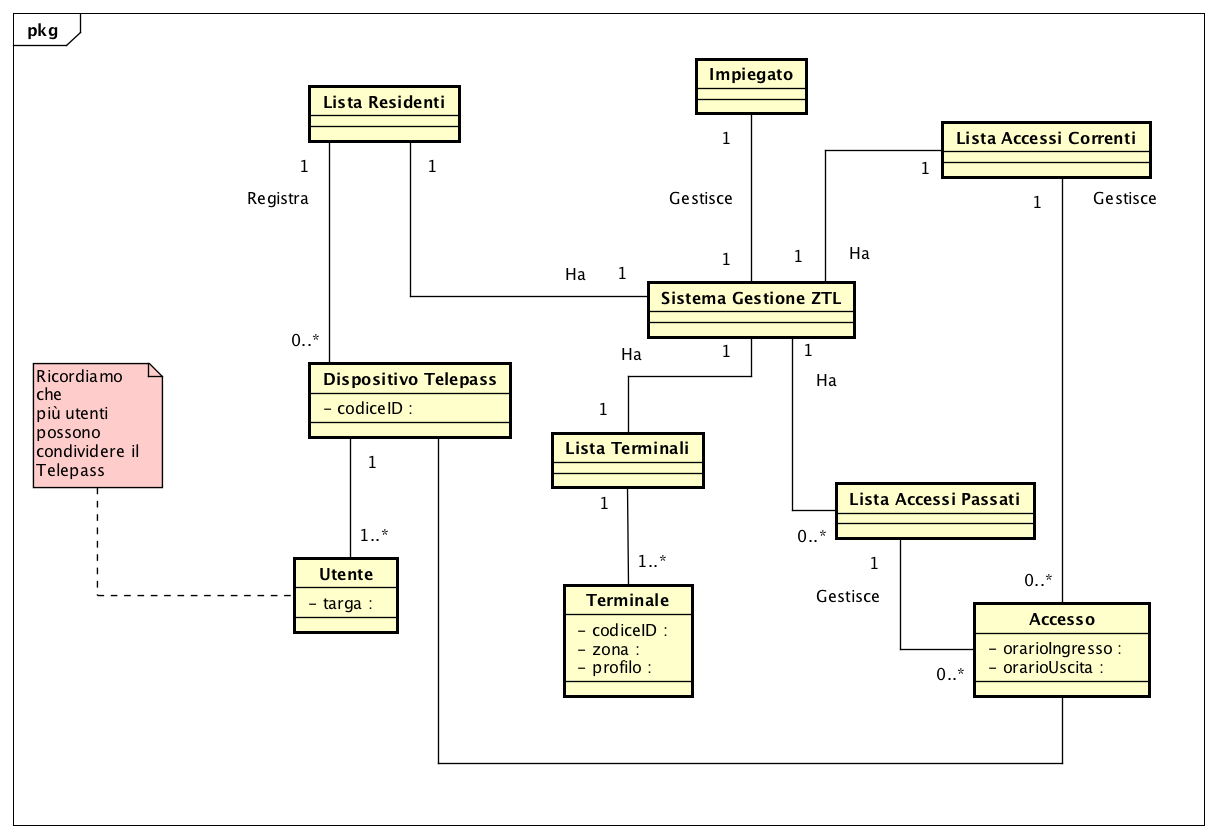
\includegraphics[scale=0.40]{ModelloDominio}
    \label{fig:mesh1}
\end{figure}

\section{Diagrammi di Sequenza di Sistema}

\subsection{UC1}
Per accomodare la presenza di utenti 
carico-scarico, il diagramma di sequenza è 
diviso in tre sezioni, che rappresentano 
i messaggi ritornati nel caso rispettivamente 
in cui l'utente sia residente, non residente con 
transito regolare e non residente con transito 
irregolare. 
\begin{figure}[H]
    \centering
    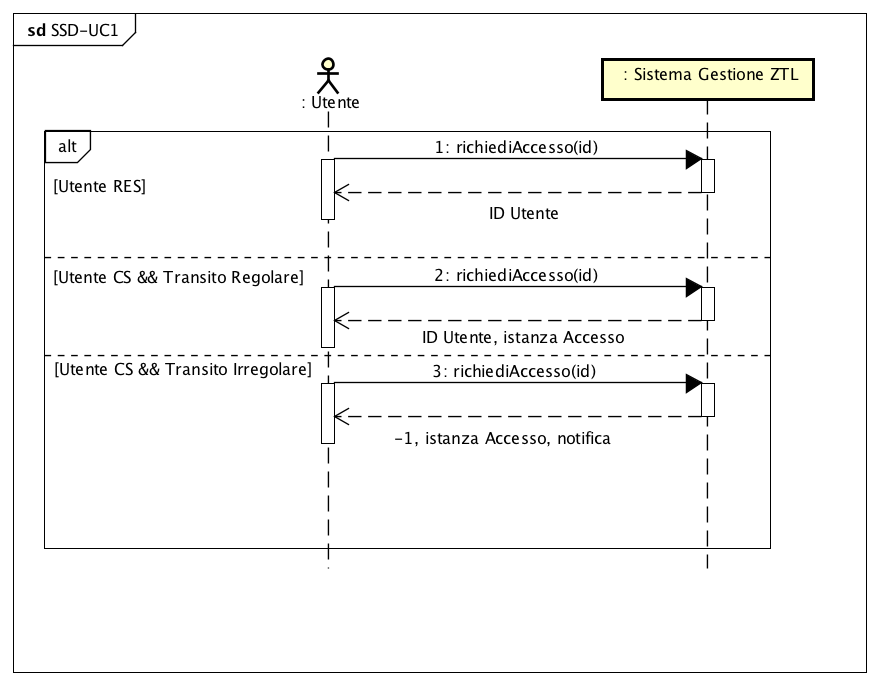
\includegraphics[scale=0.50]{SSD-UC1}
    \label{fig:mesh1}
\end{figure}

\subsection{UC2}
Come per il caso d'uso \emph{UC1}, includiamo 
nel diagramma di sequenza il caso in cui 
l'utente carico-scarico esce senza aver commesso 
irregolarità ed il caso ove invece compie 
un'irregolarità.
\begin{figure}[H]
    \centering
    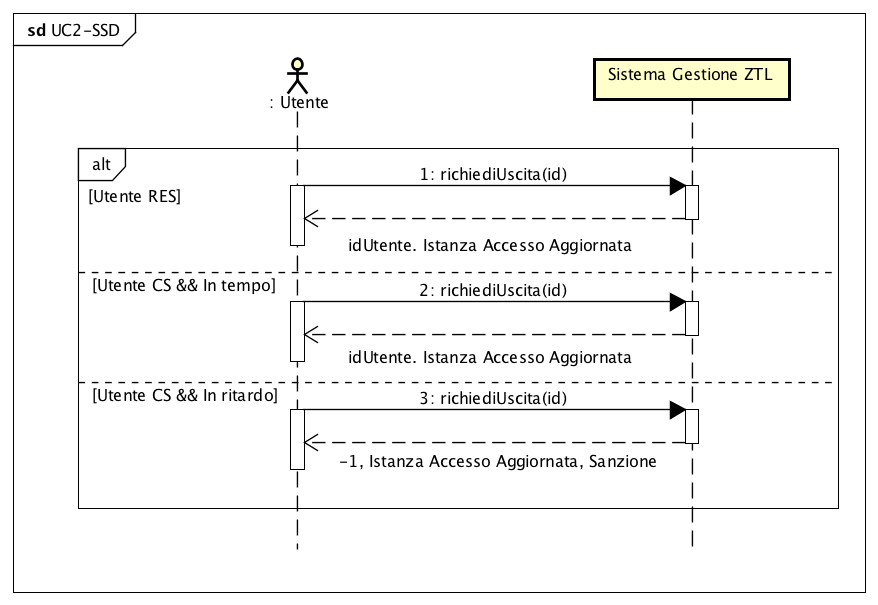
\includegraphics[scale=0.50]{SSD-UC2}
    \label{fig:mesh1}
\end{figure}

\subsection{UC3.1}
\begin{figure}[H]
    \centering
    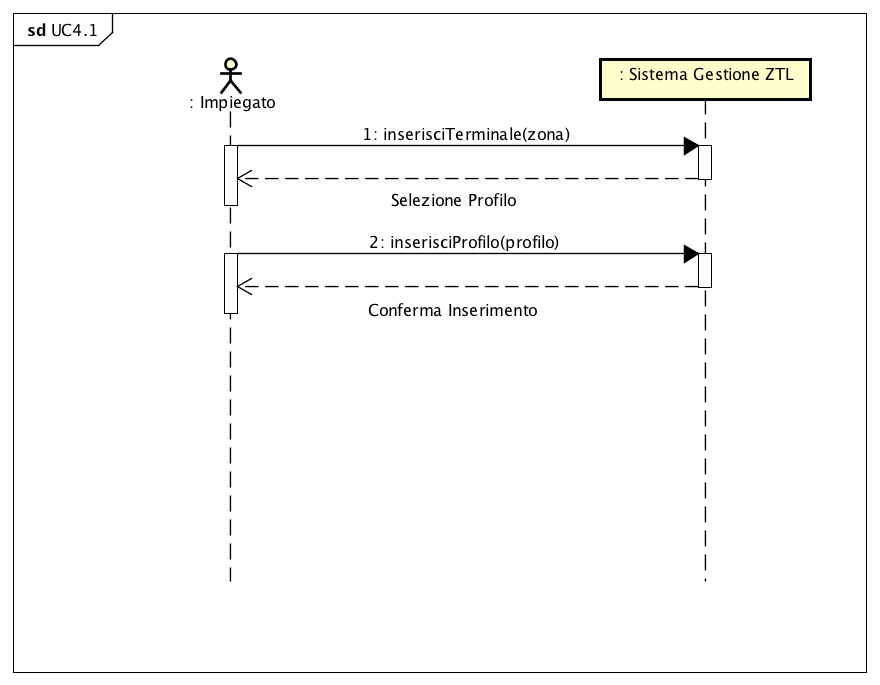
\includegraphics[scale=0.50]{SSD-UC3.1}
    \label{fig:mesh1}
\end{figure}

\subsection{UC4.1}
\begin{figure}[H]
    \centering
    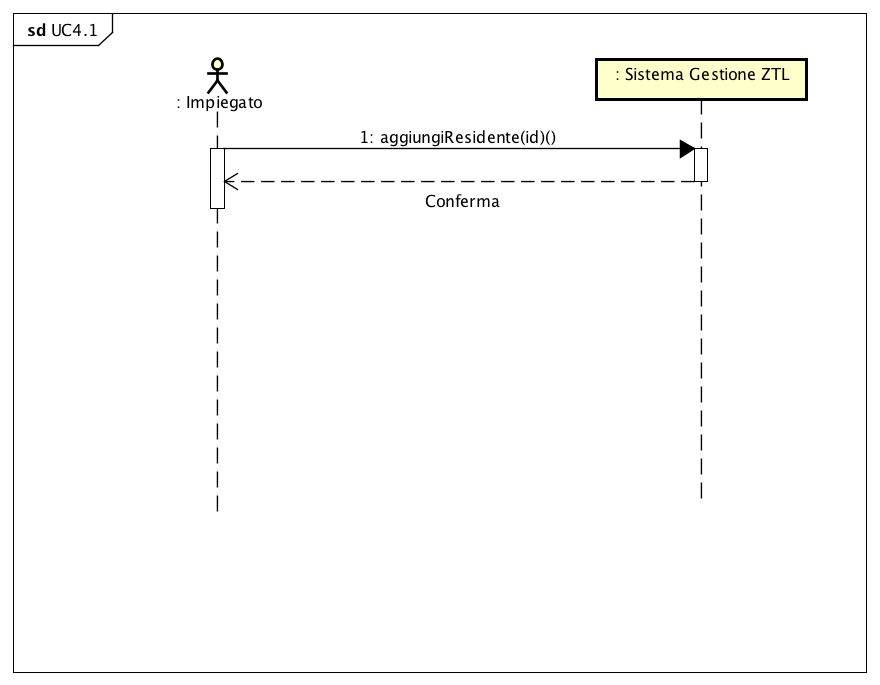
\includegraphics[scale=0.50]{SSD-UC4.1}
    \label{fig:mesh1}
\end{figure}

\section{Contratti delle operazioni}
Per accomodare gli utenti carico-scarico, modifichiamo
i contratti precedenti e le relative operazioni, dato 
che adesso gli accessi per tale tipologia di utenti devono
essere registrati

\subsection{CO1}
\begin{itemize}
    \item \textbf{Operazione:} \texttt{richiediAccesso(idUtente : int, hh : int, mm : int)}
    \item \textbf{Riferimenti:} Caso d'uso UC1
    \item \textbf{Pre-condizioni:} un utente 
    si trova in procinto di accedere
    \item \textbf{Post-condizioni:} l'utente 
    è entrato nella zona a traffico limitato
    e, se carico-scarico, l'ingresso è stato 
    registrato
\end{itemize}

\subsection{CO2}
\begin{itemize}
    \item \textbf{Operazione:} \texttt{richiediUscita(idUtente : int, hh : int, mm : int)}
    \item \textbf{Riferimenti:} Caso d'uso UC1
    \item \textbf{Pre-condizioni:} un utente 
    è procinto di uscire dalla zona a traffico limitato
    \item \textbf{Post-condizioni:} l'utente 
    è uscito dalla zona a traffico limitato e,
    se carico scarico, l'istanza d'accesso è stata 
    aggiornata e registrata nello storico degli 
    accessi
\end{itemize}

\subsection{CO3}
\begin{itemize}
    \item \textbf{Operazione:} \texttt{registraAccesso(idUtente : int, hh : int, mm : int)}
    \item \textbf{Riferimenti:} Caso d'uso UC1
    \item \textbf{Pre-condizioni:} un utente 
    carico-scarico ha eseguito l'accesso
    \item \textbf{Post-condizioni:} l'utente 
    è stato registrato nel sistema come utente 
    in transito
\end{itemize}

\subsection{CO4}
\begin{itemize}
    \item \textbf{Operazione:} \texttt{registraUscita(idUtente : int, hh : int, mm : int)}
    \item \textbf{Riferimenti:} Caso d'uso UC2
    \item \textbf{Pre-condizioni:} un utente 
    carico-scarico ha lasciato la zona a traffico 
    limitato
    \item \textbf{Post-condizioni:} l'accesso 
    viene modificato con l'orario di uscita e 
    viene inserito in uno storico di accessi
\end{itemize}

\section{Diagrammi di Interazione}
\subsection{UC1}
Riportiamo di seguito il diagramma per il Caso D'Uso 
\emph{UC1} riportando le casistiche nel caso in cui 
l'utente sia residente o carico-scarico.
\begin{figure}[H]
    \centering
    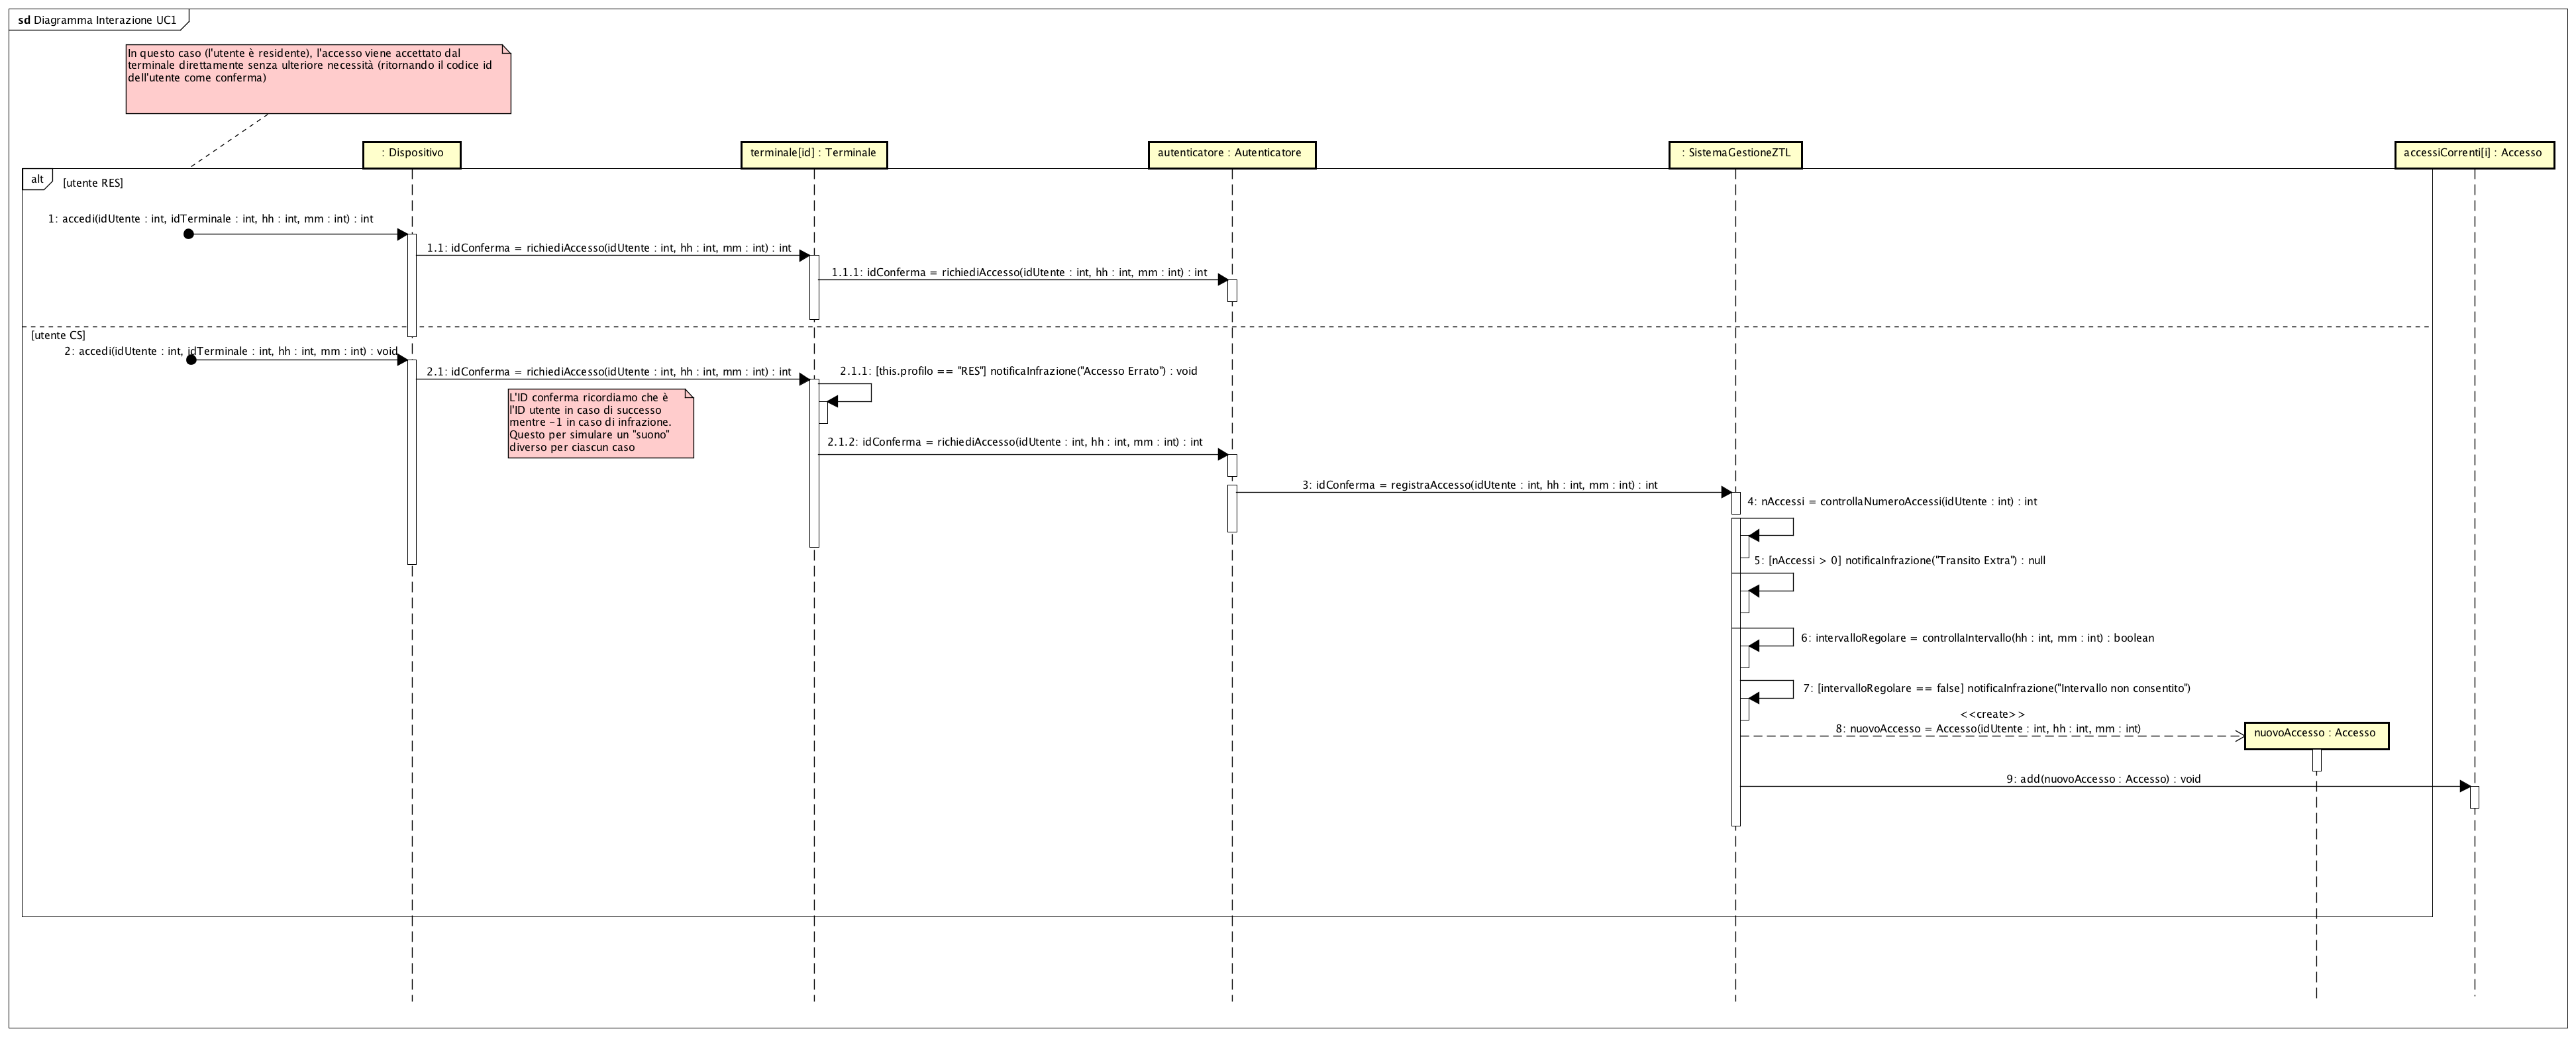
\includegraphics[scale=0.10]{DI-UC1}
    \label{fig:mesh1}
\end{figure}

\subsection{UC2}
Illustriamo di seguito il diagramma per il Caso D'Uso 
\emph{UC2} riportando anche qui le casistiche nel caso in cui 
l'utente sia residente o carico-scarico.
\begin{figure}[H]
    \centering
    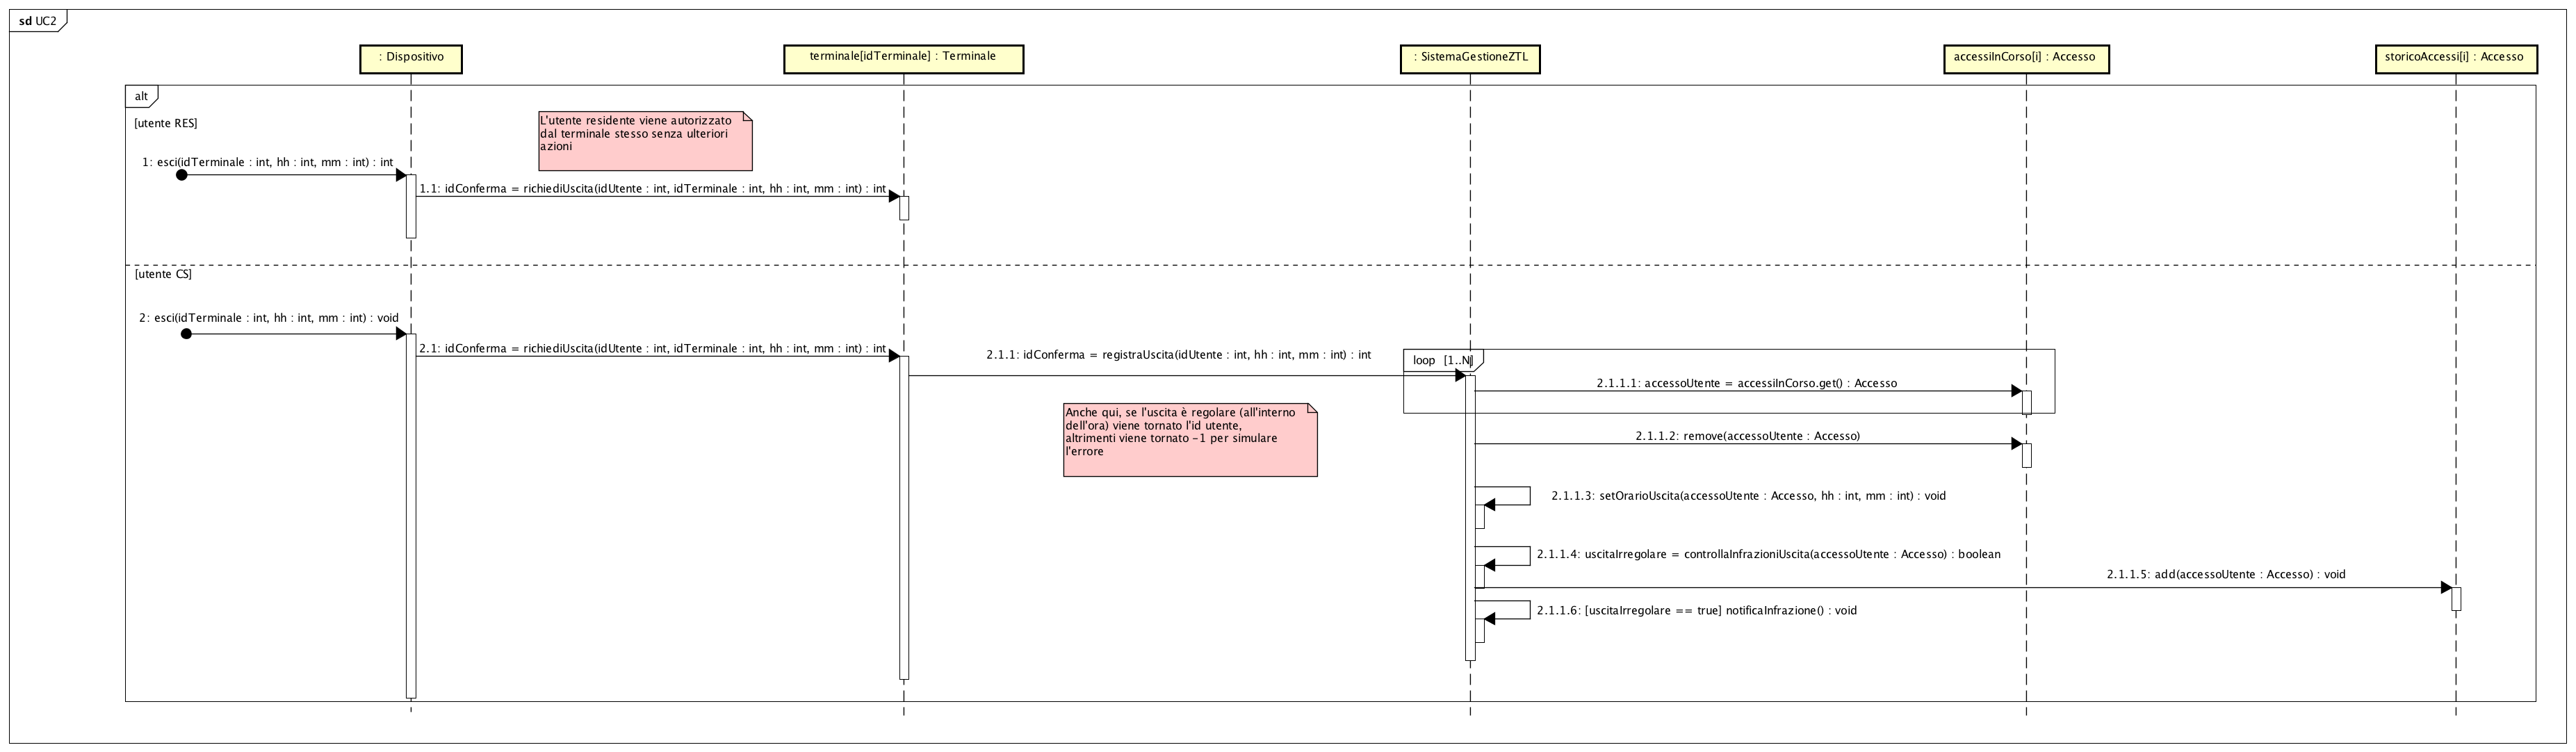
\includegraphics[scale=0.13]{DI-UC2}
    \label{fig:mesh1}
\end{figure}

\subsection{UC3.1}
Illustriamo di seguito il diagramma per il Caso D'Uso 
\emph{UC3.1 - Aggiungi Terminale}. Aggiungiamo i dati,
verifichiamo l'esistenza ed a seconda, o aggiorneremo 
il profilo, oppure creiamo un nuovo terminale e lo 
aggiungiamo.
modo per identificarlo alla ZTL.
\begin{figure}[H]
    \centering
    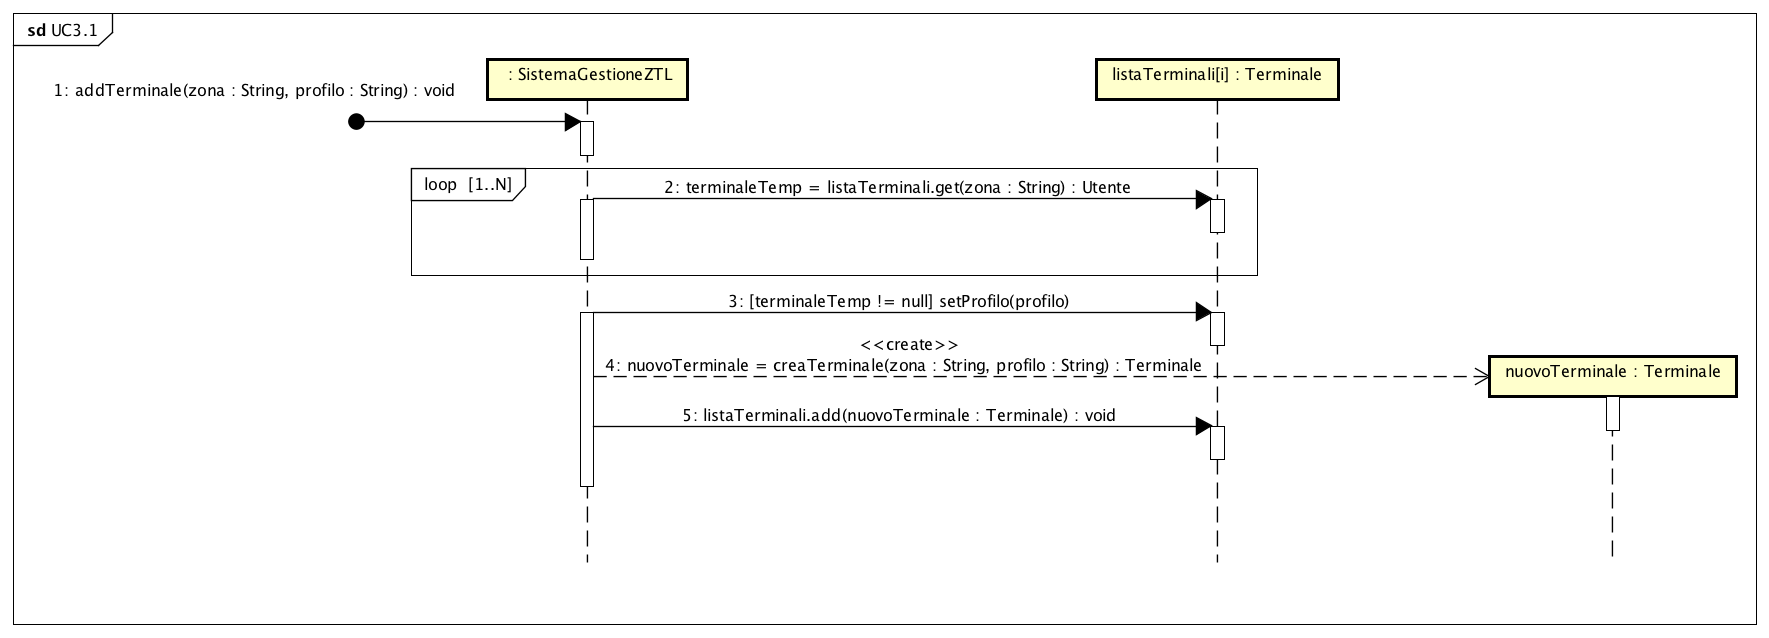
\includegraphics[scale=0.25]{DI-UC3.1}
    \label{fig:mesh1}
\end{figure}

\subsection{UC4.1}
Illustriamo di seguito il diagramma per il Caso D'Uso 
\emph{UC4.1 - Aggiungi Residente}. Notiamo che l'utente 
è di tipo \emph{Dispotivo}, in quanto esso è l'unico 
modo per identificarlo alla ZTL.
\begin{figure}[H]
    \centering
    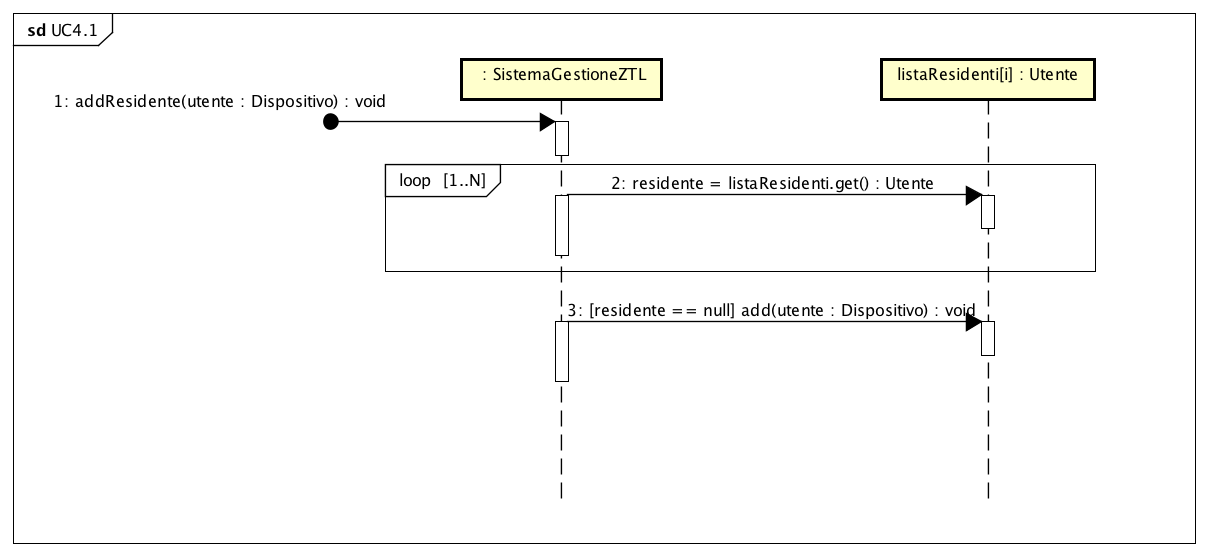
\includegraphics[scale=0.40]{DI-UC4.1}
    \label{fig:mesh1}
\end{figure}

\section{Diagramma delle Classi Progettuali}
\begin{figure}[H]
    \centering
    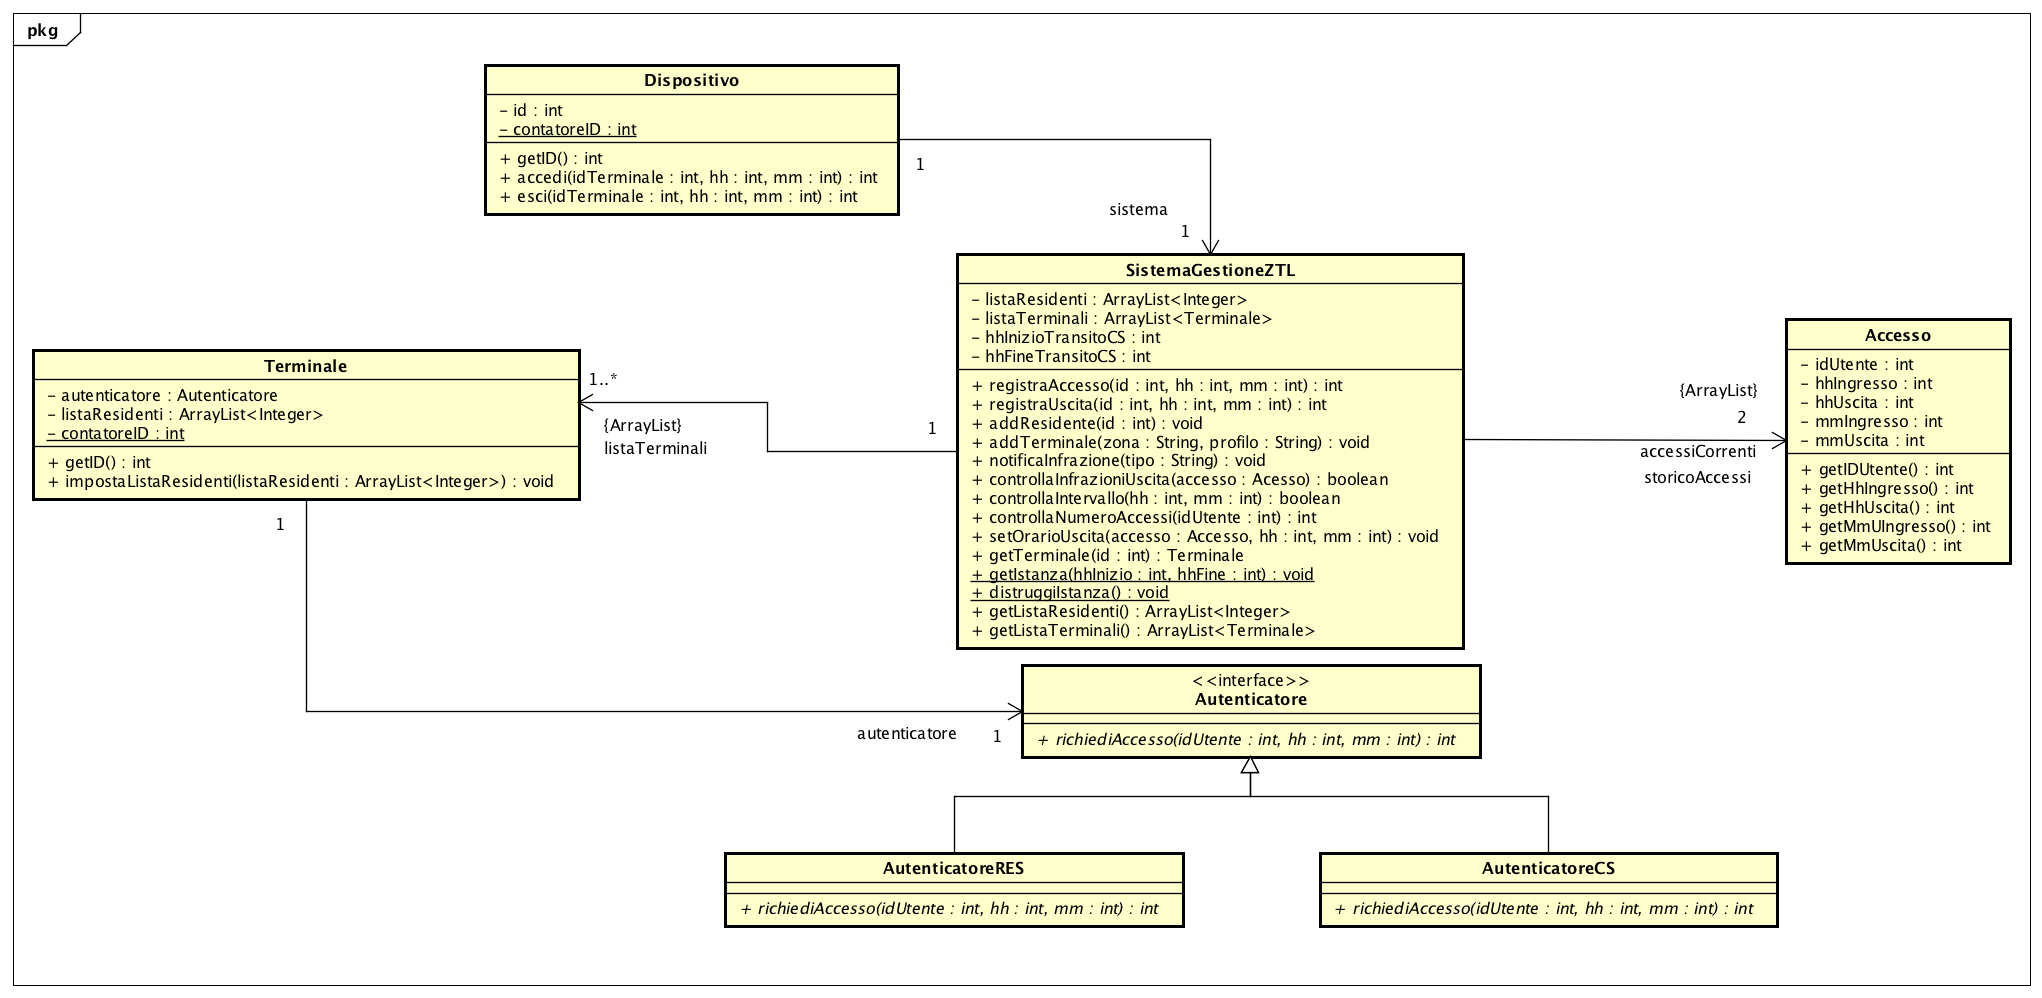
\includegraphics[scale=0.25]{DiagrammaClassi}
    \label{fig:mesh1}
\end{figure}

\section{Motivazioni progettuali}

\subsection{Meccanismo di sottoscrizione con 
pattern \emph{Observer}}
Quando un utente viene aggiunto alla lista 
dei residenti, questa deve essere aggiornata 
in tutti i terminali. Utilizziamo il pattern 
\emph{Observer} per implementare un efficace 
meccanismo di sottoscrizione dove ad ogni 
utente aggiunto, viene inviata la "notifica" 
ai terminali.

\subsection{Encapsulamento dell'algoritmo di 
riconoscimento con pattern \emph{Strategy}}
Il terminale, a seconda del profilo, implementa 
il pattern Strategy, in modo che a profili diversi 
corrispondono strategie diverse.

\subsection{Distribuzione delle responsabilità}
Utilizzando un insieme di pattern \emph{GRASP},
abbiamo voluto delegare la creazione di Terminali
e Residenti al sistema centrale dato che sembra
il più adeguato a tale mansione \emph{(Creator)}.
Stessa cosa per le istanze della classe \emph{Accesso},
che vengono delegate al sistema centrale dato che 
le registra.


\section{Casi di Test}

\subsection{Test unitari per \texttt{richiediAccesso}}
Testiamo suddetto metodo, utilizzando le seguenti
combinazioni:
\begin{itemize}
    \item Utente Residente, Terminale Residente 
    \item Utente Carico-Scarico, Terminale Residente 
    \item Utente Carico-Scarico, Terminale Carico-Scarico 
    \item Utente Residente, Terminale Carico-Scarico
\end{itemize}

\noindent
I primi due verranno eseguiti per la classe 
\emph{AutenticazioneRES}, e verrà enfatizzato
nel test il fatto che i residenti hanno accesso 
illimitato (viene fatto accedere alle 2:00 di notte)
mentre gli utenti carico scarico nemmeno 
nell'intervallo consentito (9:00-21:00) possono 
accedere.

\noindent
Gli ultimi due invece afferiscono alla classe 
\emph{AutenticazioneCS}, e testeremo che nel 
primo caso, l'ingresso alle 21:20 sia illecito e 
l'ingresso alle 11 lecito. Nel secondo caso,
alle 2 di notte, mostreremo che l'ingresso 
sia lecito.

\noindent
Per gli intervalli, testiamo un utente carico-scarico 
all'interno, all'esterno, e proprio al punto di uscita,
e ci aspetteremo che in questo ultimo caso non 
succeda nulla.

\noindent
Vogliamo anche testare un accesso multiplo di 
un utente carico-scarico in modo da verificare 
che esso venga notificato.

\subsection{Test unitari per la classe
\texttt{SistemaGestioneZTL}}
In tale classe, vogliamo verificare che 
i metodi \texttt{controllaIntervallo} e
\texttt{controllaInfrazioneUscita} siano 
esatti. In particolare, il primo deve 
ritornare \texttt{false} se l'ora data 
in input si trova al di fuori dell'intervallo 
mentre il secondo deve controllare, data
l'istanza d'accesso, che l'utente sia uscito
entro l'ora e non oltre lo scattare dell'ora:
un'ora ed un minuto è da considerarsi uscita 
irregolare.
In particolare:
\begin{itemize}
    \item La zona a traffico limitato consentirà 
    l'accesso dalle 9 alle 21. 
    \item L'orario 8:30 dovrà 
    restituire \texttt{false} alla chiamata
    a \texttt{controllaIntervallo}.
    \item L'orario 9:00 dovrà 
    restituire \texttt{true} alla chiamata
    a \texttt{controllaIntervallo}.
    \item L'orario 21:00 dovrà 
    restituire \texttt{true} alla chiamata
    a \texttt{controllaIntervallo}.
    \item Viene creato un accesso 
    alle 9:30 che esce alle 10:31.
    Tale dovrà restituire 
    \texttt{true} alla chiamata a 
    \texttt{controllaInfrazioneUscita}.
    Lo steso viene fatto uscire alle 
    10:30, e dovrà restituire 
    \emph{false}.
\end{itemize}

\subsection{Test Strutturali di Sistema}
Come al solito, il cliente (comune) eseguirà 
un test attraverso la classe \texttt{TestDriver}
usando la classe \texttt{Utente} che simula la 
vettura. In tal modo sarà lui stesso a rendersi 
conto dell'andazzo del progetto e darci un 
feedback.

\end{document}